\documentclass[12pt, a4paper]{article}

\usepackage[utf8]{inputenc}
\usepackage[russian]{babel}
\parindent 0pt
\parskip 8pt
\usepackage{amsmath}
\usepackage{amssymb}
\usepackage{array}
\usepackage[left=2.3cm, right=2.3cm, top=2.7cm, bottom=2.7cm, bindingoffset=0cm]{geometry} % headheight=0pt,
\usepackage{hyperref}
\usepackage{graphicx}
\usepackage{multicol}
\usepackage{fancyhdr} 
\usepackage{extramarks}
\usepackage[usenames,dvipsnames]{color}
\usepackage{titlesec}
\usepackage[normalem]{ulem}
\usepackage{tikz}
\definecolor{grey}{RGB}{128,128,128}

\pagestyle{fancy}
\fancyhf{}
\lhead{Билет № 1.2}
\chead{Оперативная память:\\характеристики, типы динамической памяти.}
\rhead{\thepage}
\lfoot{made with Ы}
\cfoot{}
\rfoot{\today}
\renewcommand\headrulewidth{0.4pt}
\renewcommand\footrulewidth{0.4pt}

\titlespacing*{\section}{0pt}{5pt}{0pt}
\titlespacing*{\subsection}{0pt}{5pt}{0pt}
\titlespacing*{\subsubsection}{0pt}{5pt}{0pt}

\begin{document}
\section{Обычная DRAM}
\begin{figure}[h]
    \centering
    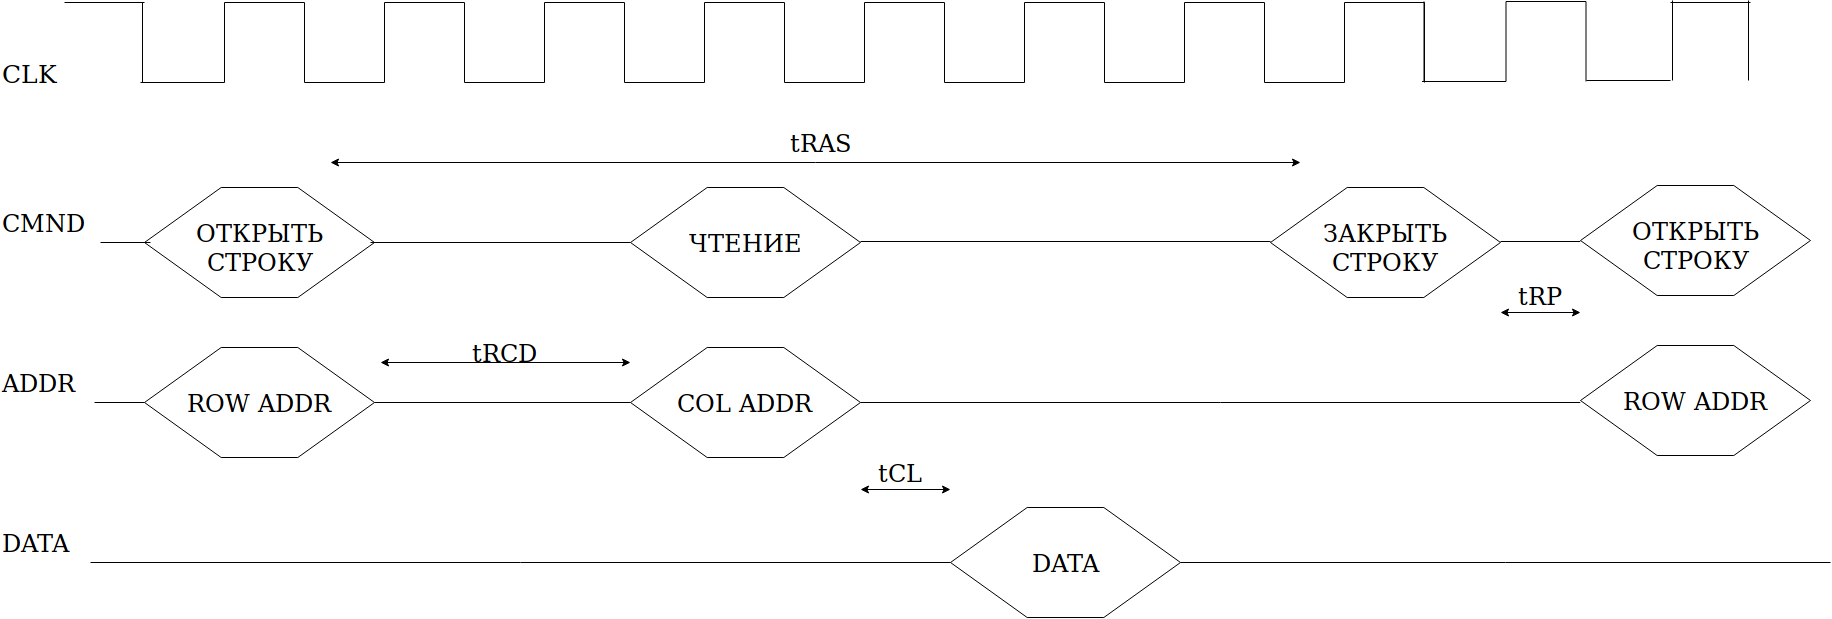
\includegraphics[scale=0.2]{images/DRAM.png}
    \caption{Схема работы DRAM}
    \label{fig:DRAM}
\end{figure}
Вернемся к устройству модуля памяти. За два такта передаём адрес. После выбора строки все ячейки этой строки считываются в отдельную маленькую статическую память. На этот момент в самом модуле в строке одни $0$, т.к. конденсаторы разрядились при чтении. Уже из статической памяти считываем столбец и всю строку записываем обратно в динамическую.\\
\textit{Внимание\_0}: эта штука \textbf{асинхронная}.\\
\textit{Внимание\_1}: адрес столбца должен быть зажат пока не получены данные.
\section{Тайминги}
\begin{itemize}
    \item \textbf{CL} - \textit{CAS (Column Address Strobe) Latency} - число тактов между отправкой адреса столбца и началом получения данных.
    \item \textbf{tRCD} - \textit{RAS (Row Address Strobe) to CAS Delay} - минимальное число тактов, которое нужно подождать при открытой строке, прежде чем открывать столбец.
    \item \textbf{tRP} - \textit{Row Precharge} - минимальное число тактов, которое нужно подождать между закрытием строки и открытием новой.
    \item \textbf{tRAS} - \textit{Row Active Strobe} - минимальное число тактов между откртием и закрытием строки.
\end{itemize}
\section{Как сравнивать два модуля памяти?}
\begin{itemize}
    \item Если частота одинаковая, то чем меньше CL, тем лучше для последовательных запросов. Чем меньше tRP + tRAS, тем лучше для случайных запросов.
    \item Если частота разная, то такты в памяти с большей частотой будут означать пропорционально меньшие промежутки времени.
\end{itemize}
\section{Характеристики памяти}
Скорость бывает двух видов: \textbf{скорость доступа} \textit{latency} и \textbf{скорость передачи данных} или \textbf{пропускная способность} \textit{throughput}.\\
\textbf{Скорость доступа} характеризует время от получения запроса до получения первой порции данных. В RAM скорость доступа = tCL + tRCD\\
\textbf{Скорость передачи данных} характеризует время от $n$-ной до $n+1$-ой порции данных. В RAM скорость передачи данных = tRAS + tRP\\
\begin{figure}[h]
    \centering
    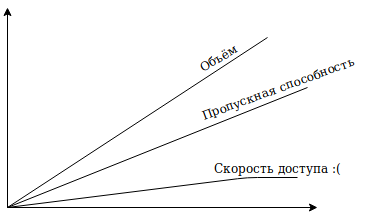
\includegraphics[scale=0.4]{./images/graphic.png}
    \caption{График, показывающий как изменялись характеристики памяти с течением времени}
    \label{fig:SDR_SDRAM}
\end{figure}
Как видно из графика, со скоростью доступа всё очень грустно.
\section{Важная информация}
Память - \textit{пассивное} устройство. Процессор \textit{запрашивает}, память \textit{отвечает на запрос}.
\section{FPM DRAM}
\textbf{FPM DRAM} - textit{Fast Page Mode DRAM} - а давайте закрывать строку не каждый раз, а только когда следующий запрос идет в другую строку. Т.е. читать столбцы одной строки без закрытия этой строки.\\
Улучшилась скорость передачи\\
\textit{Внимание\_0}: эта штука \textbf{асинхронная}.\\
\textit{Внимание\_1}: адрес столбца должен быть зажат пока не получены данные.
\section{EDO DRAM}
\textbf{EDO DRAM} - \textit{Enabled Data Out DRAM} - а давайте добавим буфер для адреса столбца. Теперь пока читается один столбец, мы можем уже подать адрес следующего, а после получения данных с первого столбца, сигнал на чтение второго.\\
Улучшилась скорость передачи.\\
\textit{Внимание}: эта штука всё ещё \textbf{асинхронная}.
\section{BEDO DRAM}
\textbf{BEDO DRAM} - \textit{Burst EDO DRAM} - теперь на запрос чтения столбца память отдаёт не только нужный столбец, но и три следующих. Ограничения: адрес должен быть кратен четырем.\\
Улучшилась скорость передачи.\\
\textit{Внимание}: эта штука всё ещё \textbf{асинхронная}.
\section{SDRAM}
До появления SDRAM контроллер память и модуль памяти \textit{не были синхронизированы}. У них даже могли быть разные частоты.\\
Пусть у нас tRCD - 3 такта. Но контроллеру приходилось ждать "с запасом".\\
\textbf{SDRAM} - \textit{Synchronious DRAM} - теперь контроллер и память на одной синхронизации. Следовательно контроллер может ждать ровно tRCD тактов.\\
Кроме того, в SDRAM увеличили ширину шины до 64 бит и появились \textbf{банки памяти} (от 2 до 4).\\
За счет поджатия таймингов и увеличения ширины шины увеличилась скорость передачи.\\
Внутренняя и внешняя шина SDR SDRAM работают на одной частоте. Если хочется, чтобы память работала быстрее, нужно поднимать частоты. А поднимать частоты достаточно грустно, потому что растет энергопотребление и тепловыделение.
\begin{figure}[h]
    \centering
    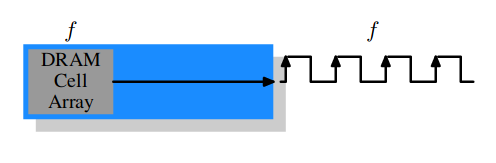
\includegraphics[scale=0.6]{./images/SDR_SDRAM.png}
    \caption{\textbf{SDR SDRAM} - Single Data Rate SDRAM}
    \label{fig:SDR_SDRAM}
\end{figure}
\section{Еще немного про модули памяти}
Процессор явно работает быстрее, чем память. Следовательно у памяти рано или поздно появится очередь запросов. Хотелось бы сделать такую память, которая может обрабатывать запросы параллельно.
\subsection{Многопортовая память}
\begin{figure}[h]
    \centering
    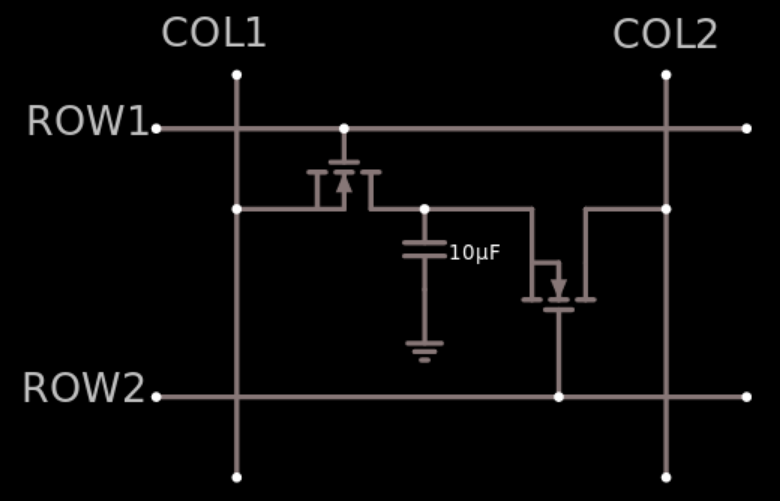
\includegraphics[scale=0.3]{./images/MultiportDRAM.png}
    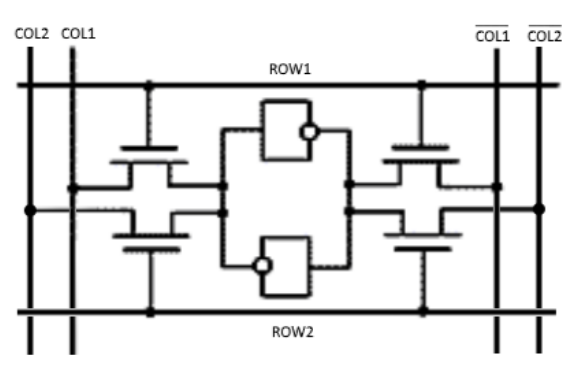
\includegraphics[scale=0.3]{./images/MultiportSRAM.png}
    \caption{Двухпортовые ячейки DRAM(слева) и SRAM(справа)}
    \label{fig:MultiportMEM}
\end{figure}
При таком подходе к каждой ячейке подходит два набора линий строки/столбца.\\
Идейно мы как будто бы обращаемся к двум разным матрицам, заполненным одинаковыми данными. \textbf{НО!} Мы не можем обратиться одновременно к одной и той же строке.\\
Улучшается время доступа к разным строкам.\\
На практике используется в SRAM, а в DRAM нет.
\subsection{Многобанковая память}
Идейно среднее между однобанковой и многобанковой памятью)000))))\\
\begin{figure}[h]
    \centering
    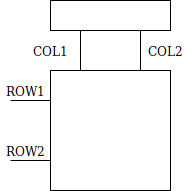
\includegraphics[scale=0.45]{./images/MultiportMEM.png}
    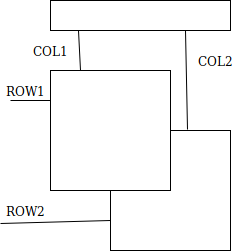
\includegraphics[scale=0.45]{./images/MultibankMEM.png}
    \caption{Модуль многопортовой и многобанковой памяти}
    \label{fig:MultiportMEM}
\end{figure}
При таком подходе используем действительно две разных матрицы. Усложняется только интерфейсная схема, а сами ячейки остаются простыми.\\
В итоге получаем улучшения при работе со строками, лежащими в разных банках памяти.
\subsection{Многоканальный режим работы}
Пусть есть sdram c шиной 64 бита.
Втыкаем в оба канала модуль памяти. Теперь шина 128 бит.
Желательно чтобы модули памяти были максимально похожи. Лучше чтобы они были одинакового объема, иначе контроллер может сказать "не, я так не умею"" и рабоать в одноканальном режиме. 
\section{DDR}
\textbf{DDR SDRAM} - \textit{Double Data Rate SDRAM} - увеличили внутреннюю шину в два раза, а ширину внешней оставили прежней. Можем передавать данные два раза за такт: по фронту и по спаду импульса синхронизации. (На пересечении прямого и инвертированного импульса синхронизации)\\
\textbf{Маркетинговая уловка:} а давайте введем понятие эффективной частоты (на какой частоте нужно было бы работать старому модулю памяти, чтобы передавать столько же информации). Нормальная частота не поменялась, но теперь можно говорить, что эффективная частота в два раза выше, чем раньше. Такие дела.
\begin{figure}[h]
    \centering
    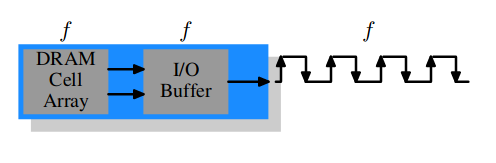
\includegraphics[scale=0.6]{./images/DDR_SDRAM.png}
    \caption{DDR SDRAM}
    \label{fig:DDR_SDRAM}
\end{figure}
\section{DDR2}
Еще раз увеличили ширину внутренней шины в два раза, и подняли частоту внешней в два раза. Снизили напряжение питания. 
\begin{figure}[h]
    \centering
    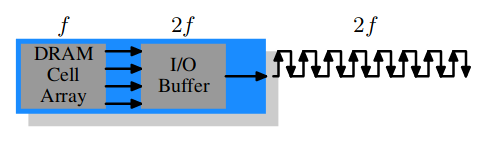
\includegraphics[scale=0.6]{./images/DDR2_SDRAM.png}
    \caption{DDR2 SDRAM}
    \label{fig:DDR2_SDRAM}
\end{figure}
\section{DDR3}
Еще раз увеличили ширину внутренней шины в два раза, и подняли частоту внешней в два раза. Снизили напряжение питания.
\begin{figure}[h]
    \centering
    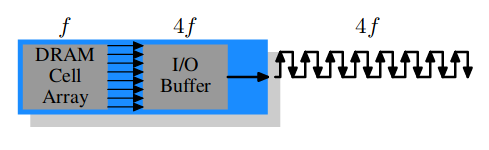
\includegraphics[scale=0.6]{./images/DDR3_SDRAM.png}
    \caption{DDR3 SDRAM}
    \label{fig:DDR2_SDRAM}
\end{figure}
\section{DDR4}
\sout{Еще раз увеличили ширину внутренней шины...} А вот и нет. Дальше увеличивать ширину внутренней шины уже слишком жирно (там и так $8n$ проводов, если в SDRAM $n$). Поэтому только уменьшили напряжение питания.\\
\section{GDDR}
\textbf{Graphic DDR} - оптимизирована на высокую скорость передачи данных. Сильно греются, имеют высокую тактовую частоту.\\
GDDR3 ~ DDR2
GDDR5 ~ DDR3, вроде как однопортовая, но хорошо притворяется двухпортовой из-за внутренних хаков.
GDDR5X ~ DDR3
\section{HBM память*}
Особая технология подключения памяти к процессору. Используется в топовых видеокарточках. Ширина шины сильно больше. Но технология сильно дороже и сложнее, чем обычные печатные платы.
\begin{figure}[h!]
    \centering
    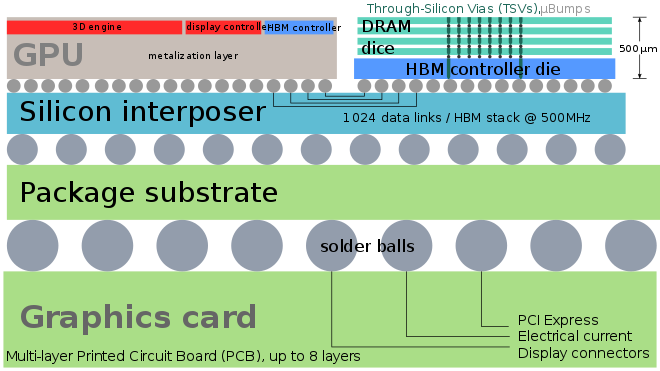
\includegraphics[scale=0.4]{./images/HBM.png}
    \caption{Технология HBM в разрезе}
    \label{fig:HBM}
\end{figure}
\section{Источники}
\begin{itemize}
    \item Википедия
    \item конспекты лекций by @ntwwwnt
    \item "What Every Programmer Should Know About Memory" by Ulrich Drepper
\end{itemize}
\end{document}